% Generated by Sphinx.
\def\sphinxdocclass{report}
\documentclass[letterpaper,10pt,french]{sphinxmanual}
\usepackage[utf8]{inputenc}
\DeclareUnicodeCharacter{00A0}{\nobreakspace}
\usepackage{cmap}
\usepackage[T1]{fontenc}
\usepackage{babel}
\usepackage{times}
\usepackage[Sonny]{fncychap}
\usepackage{longtable}
\usepackage{sphinx}
\usepackage{multirow}

\addto\captionsfrench{\renewcommand{\figurename}{Fig. }}
\addto\captionsfrench{\renewcommand{\tablename}{Tableau }}
\floatname{literal-block}{Code source }



\title{GICO Documentation}
\date{07 July 2015}
\release{1.0.0}
\author{Gicoteurs}
\newcommand{\sphinxlogo}{}
\renewcommand{\releasename}{Version}
\makeindex

\makeatletter
\def\PYG@reset{\let\PYG@it=\relax \let\PYG@bf=\relax%
    \let\PYG@ul=\relax \let\PYG@tc=\relax%
    \let\PYG@bc=\relax \let\PYG@ff=\relax}
\def\PYG@tok#1{\csname PYG@tok@#1\endcsname}
\def\PYG@toks#1+{\ifx\relax#1\empty\else%
    \PYG@tok{#1}\expandafter\PYG@toks\fi}
\def\PYG@do#1{\PYG@bc{\PYG@tc{\PYG@ul{%
    \PYG@it{\PYG@bf{\PYG@ff{#1}}}}}}}
\def\PYG#1#2{\PYG@reset\PYG@toks#1+\relax+\PYG@do{#2}}

\expandafter\def\csname PYG@tok@gd\endcsname{\def\PYG@tc##1{\textcolor[rgb]{0.63,0.00,0.00}{##1}}}
\expandafter\def\csname PYG@tok@gu\endcsname{\let\PYG@bf=\textbf\def\PYG@tc##1{\textcolor[rgb]{0.50,0.00,0.50}{##1}}}
\expandafter\def\csname PYG@tok@gt\endcsname{\def\PYG@tc##1{\textcolor[rgb]{0.00,0.27,0.87}{##1}}}
\expandafter\def\csname PYG@tok@gs\endcsname{\let\PYG@bf=\textbf}
\expandafter\def\csname PYG@tok@gr\endcsname{\def\PYG@tc##1{\textcolor[rgb]{1.00,0.00,0.00}{##1}}}
\expandafter\def\csname PYG@tok@cm\endcsname{\let\PYG@it=\textit\def\PYG@tc##1{\textcolor[rgb]{0.25,0.50,0.56}{##1}}}
\expandafter\def\csname PYG@tok@vg\endcsname{\def\PYG@tc##1{\textcolor[rgb]{0.73,0.38,0.84}{##1}}}
\expandafter\def\csname PYG@tok@m\endcsname{\def\PYG@tc##1{\textcolor[rgb]{0.13,0.50,0.31}{##1}}}
\expandafter\def\csname PYG@tok@mh\endcsname{\def\PYG@tc##1{\textcolor[rgb]{0.13,0.50,0.31}{##1}}}
\expandafter\def\csname PYG@tok@cs\endcsname{\def\PYG@tc##1{\textcolor[rgb]{0.25,0.50,0.56}{##1}}\def\PYG@bc##1{\setlength{\fboxsep}{0pt}\colorbox[rgb]{1.00,0.94,0.94}{\strut ##1}}}
\expandafter\def\csname PYG@tok@ge\endcsname{\let\PYG@it=\textit}
\expandafter\def\csname PYG@tok@vc\endcsname{\def\PYG@tc##1{\textcolor[rgb]{0.73,0.38,0.84}{##1}}}
\expandafter\def\csname PYG@tok@il\endcsname{\def\PYG@tc##1{\textcolor[rgb]{0.13,0.50,0.31}{##1}}}
\expandafter\def\csname PYG@tok@go\endcsname{\def\PYG@tc##1{\textcolor[rgb]{0.20,0.20,0.20}{##1}}}
\expandafter\def\csname PYG@tok@cp\endcsname{\def\PYG@tc##1{\textcolor[rgb]{0.00,0.44,0.13}{##1}}}
\expandafter\def\csname PYG@tok@gi\endcsname{\def\PYG@tc##1{\textcolor[rgb]{0.00,0.63,0.00}{##1}}}
\expandafter\def\csname PYG@tok@gh\endcsname{\let\PYG@bf=\textbf\def\PYG@tc##1{\textcolor[rgb]{0.00,0.00,0.50}{##1}}}
\expandafter\def\csname PYG@tok@ni\endcsname{\let\PYG@bf=\textbf\def\PYG@tc##1{\textcolor[rgb]{0.84,0.33,0.22}{##1}}}
\expandafter\def\csname PYG@tok@nl\endcsname{\let\PYG@bf=\textbf\def\PYG@tc##1{\textcolor[rgb]{0.00,0.13,0.44}{##1}}}
\expandafter\def\csname PYG@tok@nn\endcsname{\let\PYG@bf=\textbf\def\PYG@tc##1{\textcolor[rgb]{0.05,0.52,0.71}{##1}}}
\expandafter\def\csname PYG@tok@no\endcsname{\def\PYG@tc##1{\textcolor[rgb]{0.38,0.68,0.84}{##1}}}
\expandafter\def\csname PYG@tok@na\endcsname{\def\PYG@tc##1{\textcolor[rgb]{0.25,0.44,0.63}{##1}}}
\expandafter\def\csname PYG@tok@nb\endcsname{\def\PYG@tc##1{\textcolor[rgb]{0.00,0.44,0.13}{##1}}}
\expandafter\def\csname PYG@tok@nc\endcsname{\let\PYG@bf=\textbf\def\PYG@tc##1{\textcolor[rgb]{0.05,0.52,0.71}{##1}}}
\expandafter\def\csname PYG@tok@nd\endcsname{\let\PYG@bf=\textbf\def\PYG@tc##1{\textcolor[rgb]{0.33,0.33,0.33}{##1}}}
\expandafter\def\csname PYG@tok@ne\endcsname{\def\PYG@tc##1{\textcolor[rgb]{0.00,0.44,0.13}{##1}}}
\expandafter\def\csname PYG@tok@nf\endcsname{\def\PYG@tc##1{\textcolor[rgb]{0.02,0.16,0.49}{##1}}}
\expandafter\def\csname PYG@tok@si\endcsname{\let\PYG@it=\textit\def\PYG@tc##1{\textcolor[rgb]{0.44,0.63,0.82}{##1}}}
\expandafter\def\csname PYG@tok@s2\endcsname{\def\PYG@tc##1{\textcolor[rgb]{0.25,0.44,0.63}{##1}}}
\expandafter\def\csname PYG@tok@vi\endcsname{\def\PYG@tc##1{\textcolor[rgb]{0.73,0.38,0.84}{##1}}}
\expandafter\def\csname PYG@tok@nt\endcsname{\let\PYG@bf=\textbf\def\PYG@tc##1{\textcolor[rgb]{0.02,0.16,0.45}{##1}}}
\expandafter\def\csname PYG@tok@nv\endcsname{\def\PYG@tc##1{\textcolor[rgb]{0.73,0.38,0.84}{##1}}}
\expandafter\def\csname PYG@tok@s1\endcsname{\def\PYG@tc##1{\textcolor[rgb]{0.25,0.44,0.63}{##1}}}
\expandafter\def\csname PYG@tok@gp\endcsname{\let\PYG@bf=\textbf\def\PYG@tc##1{\textcolor[rgb]{0.78,0.36,0.04}{##1}}}
\expandafter\def\csname PYG@tok@sh\endcsname{\def\PYG@tc##1{\textcolor[rgb]{0.25,0.44,0.63}{##1}}}
\expandafter\def\csname PYG@tok@ow\endcsname{\let\PYG@bf=\textbf\def\PYG@tc##1{\textcolor[rgb]{0.00,0.44,0.13}{##1}}}
\expandafter\def\csname PYG@tok@sx\endcsname{\def\PYG@tc##1{\textcolor[rgb]{0.78,0.36,0.04}{##1}}}
\expandafter\def\csname PYG@tok@bp\endcsname{\def\PYG@tc##1{\textcolor[rgb]{0.00,0.44,0.13}{##1}}}
\expandafter\def\csname PYG@tok@c1\endcsname{\let\PYG@it=\textit\def\PYG@tc##1{\textcolor[rgb]{0.25,0.50,0.56}{##1}}}
\expandafter\def\csname PYG@tok@kc\endcsname{\let\PYG@bf=\textbf\def\PYG@tc##1{\textcolor[rgb]{0.00,0.44,0.13}{##1}}}
\expandafter\def\csname PYG@tok@c\endcsname{\let\PYG@it=\textit\def\PYG@tc##1{\textcolor[rgb]{0.25,0.50,0.56}{##1}}}
\expandafter\def\csname PYG@tok@mf\endcsname{\def\PYG@tc##1{\textcolor[rgb]{0.13,0.50,0.31}{##1}}}
\expandafter\def\csname PYG@tok@err\endcsname{\def\PYG@bc##1{\setlength{\fboxsep}{0pt}\fcolorbox[rgb]{1.00,0.00,0.00}{1,1,1}{\strut ##1}}}
\expandafter\def\csname PYG@tok@mb\endcsname{\def\PYG@tc##1{\textcolor[rgb]{0.13,0.50,0.31}{##1}}}
\expandafter\def\csname PYG@tok@ss\endcsname{\def\PYG@tc##1{\textcolor[rgb]{0.32,0.47,0.09}{##1}}}
\expandafter\def\csname PYG@tok@sr\endcsname{\def\PYG@tc##1{\textcolor[rgb]{0.14,0.33,0.53}{##1}}}
\expandafter\def\csname PYG@tok@mo\endcsname{\def\PYG@tc##1{\textcolor[rgb]{0.13,0.50,0.31}{##1}}}
\expandafter\def\csname PYG@tok@kd\endcsname{\let\PYG@bf=\textbf\def\PYG@tc##1{\textcolor[rgb]{0.00,0.44,0.13}{##1}}}
\expandafter\def\csname PYG@tok@mi\endcsname{\def\PYG@tc##1{\textcolor[rgb]{0.13,0.50,0.31}{##1}}}
\expandafter\def\csname PYG@tok@kn\endcsname{\let\PYG@bf=\textbf\def\PYG@tc##1{\textcolor[rgb]{0.00,0.44,0.13}{##1}}}
\expandafter\def\csname PYG@tok@o\endcsname{\def\PYG@tc##1{\textcolor[rgb]{0.40,0.40,0.40}{##1}}}
\expandafter\def\csname PYG@tok@kr\endcsname{\let\PYG@bf=\textbf\def\PYG@tc##1{\textcolor[rgb]{0.00,0.44,0.13}{##1}}}
\expandafter\def\csname PYG@tok@s\endcsname{\def\PYG@tc##1{\textcolor[rgb]{0.25,0.44,0.63}{##1}}}
\expandafter\def\csname PYG@tok@kp\endcsname{\def\PYG@tc##1{\textcolor[rgb]{0.00,0.44,0.13}{##1}}}
\expandafter\def\csname PYG@tok@w\endcsname{\def\PYG@tc##1{\textcolor[rgb]{0.73,0.73,0.73}{##1}}}
\expandafter\def\csname PYG@tok@kt\endcsname{\def\PYG@tc##1{\textcolor[rgb]{0.56,0.13,0.00}{##1}}}
\expandafter\def\csname PYG@tok@sc\endcsname{\def\PYG@tc##1{\textcolor[rgb]{0.25,0.44,0.63}{##1}}}
\expandafter\def\csname PYG@tok@sb\endcsname{\def\PYG@tc##1{\textcolor[rgb]{0.25,0.44,0.63}{##1}}}
\expandafter\def\csname PYG@tok@k\endcsname{\let\PYG@bf=\textbf\def\PYG@tc##1{\textcolor[rgb]{0.00,0.44,0.13}{##1}}}
\expandafter\def\csname PYG@tok@se\endcsname{\let\PYG@bf=\textbf\def\PYG@tc##1{\textcolor[rgb]{0.25,0.44,0.63}{##1}}}
\expandafter\def\csname PYG@tok@sd\endcsname{\let\PYG@it=\textit\def\PYG@tc##1{\textcolor[rgb]{0.25,0.44,0.63}{##1}}}

\def\PYGZbs{\char`\\}
\def\PYGZus{\char`\_}
\def\PYGZob{\char`\{}
\def\PYGZcb{\char`\}}
\def\PYGZca{\char`\^}
\def\PYGZam{\char`\&}
\def\PYGZlt{\char`\<}
\def\PYGZgt{\char`\>}
\def\PYGZsh{\char`\#}
\def\PYGZpc{\char`\%}
\def\PYGZdl{\char`\$}
\def\PYGZhy{\char`\-}
\def\PYGZsq{\char`\'}
\def\PYGZdq{\char`\"}
\def\PYGZti{\char`\~}
% for compatibility with earlier versions
\def\PYGZat{@}
\def\PYGZlb{[}
\def\PYGZrb{]}
\makeatother

\renewcommand\PYGZsq{\textquotesingle}

\begin{document}

\maketitle
\tableofcontents
\phantomsection\label{index::doc}


L'objectif de cette documentation produit est de détailler les différentes possibilités de l'outil GICO.

GICO, pour Gestion des Inscriptions aux Cours Optionnels est une application Web permettant aux facultés de simplifier la gestion des inscription administratives aux Unités d'Enseignement optionnelles. Elle permet une pré-inscription des étudiants et une gestion automatique des capacités en fonction des groupes définis par l'administrateur. Elle permet ainsi de simplifier grandement la gestion de ce type d'enseignements.


\chapter{Documentation administrateur}
\label{index:documentation-administrateur}\label{index:documentation-du-projet-gico}
L'administrateur est la personne configurant l'application en début d'année.


\section{Utiliser le tableau de bord}
\label{admin::doc}\label{admin:utiliser-le-tableau-de-bord}
Le tableau de bord est un point d'accès rapide aux différentes informations de l'application.

\begin{notice}{note}{Note:}
En cas d'utilisateurs en attente de validation, l'interface vous le signale par la présence d'un bandeau rouge en en-tête. Se référer à la partie Gestion des utilisateurs pour davantage d'information sur la validation de comptes utilisateurs.
\end{notice}

En haut du tableau de bord, deux widgets sont présent et vous permettent d'accéder aux modules ``Au quotidien'' et ``Synthèse''. Davantage d'information sur ces modules sont présentes dans la ``Documentation professeur/secrétariat''.

La ligne du dessous regroupe des statistiques sur les différentes données saisies dans l'application (nombre de périodes, aperçu de la hiérarchie universitaire, nombre de modules et d'utilisateurs).
\begin{figure}[htbp]
\centering
\capstart

\scalebox{0.800000}{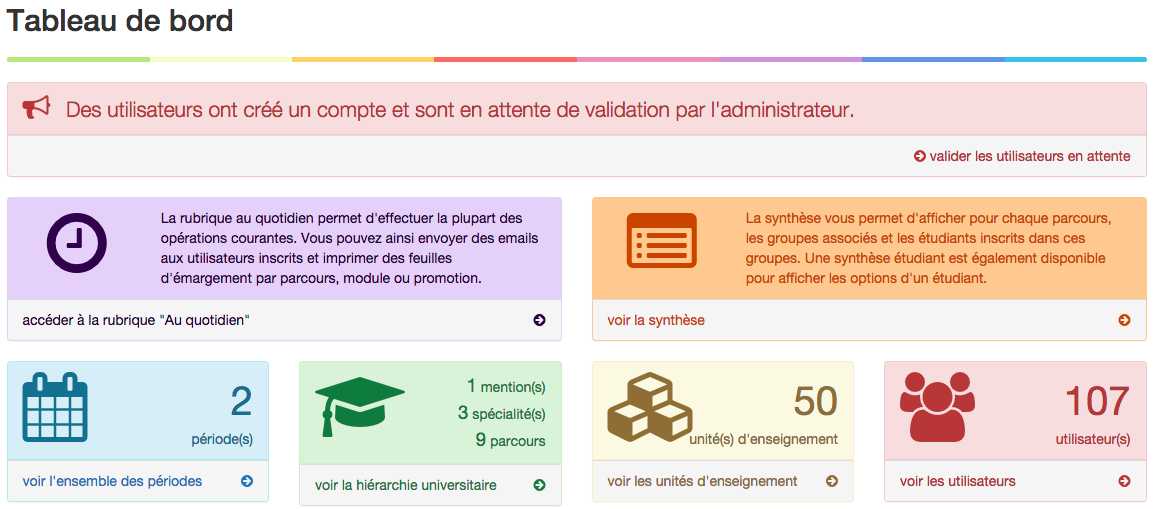
\includegraphics{dashboard.png}}
\caption{Le tableau de bord accessible à l'administrateur.}\end{figure}


\section{Créer la hiérarchie universitaire}
\label{admin:creer-la-hierarchie-universitaire}
La première chose à faire est de créer ce que nous avons appelé la ``hiérarchie universitaire''. La hiérarchie universitaire définie les diplômes et formations.
\begin{figure}[htbp]
\centering
\capstart

\scalebox{0.500000}{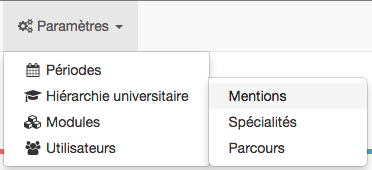
\includegraphics{menu_hierarchie.png}}
\caption{Le menu permettant d'accéder au paramétrage de la hiérarchie universitaire.}\end{figure}


\subsection{Mentions}
\label{admin:mentions}
Les mentions sont tout en haut de la hiérarchie et représentent le Master. Par exemple, STIC ou encore SANTÉ.


\subsection{Spécialités}
\label{admin:specialites}
Les spécialités représentent une spécialisation du Master. Par exemple, pour le Master STIC, les mentions MIAGE, ISIR ou 2IBS représentent les spécialités.


\subsection{Parcours}
\label{admin:parcours}
Au sein d'une même spécialité peuvent être présents différents parcours. Les parcours permettent de différencier certains enseignements au sein d'une même spécialité.

Ainsi, pour le Master STIC MIAGE, on aura les parcours :
\begin{itemize}
\item {} 
Tronc commun (année 1),

\item {} 
OSIE (année 2)

\item {} 
2COM (année 2)

\item {} 
SIS (année 2)

\end{itemize}

\begin{notice}{note}{Note:}
Le parcours étant l'élément terminal de la hiérarchie universitaire dans GICO, il doit être systématiquement présent. Si une spécialité ne comporte pas de parcours, créez tout de même un parcours ``tronc commun''.
\end{notice}


\section{Créer les périodes}
\label{admin:creer-les-periodes}
Les périodes servent à déterminer de quand à quand ont lieu les enseignement et les dates entre lesquelles les utilisateurs peuvent effectuer leurs choix.

Il est possible de créer autant de période que nécessaire. Chaque période pourra ensuite être associée à des groupes qui composeront les unitées d'enseignement. Une même période peut-être utilisée pour plusieurs groupes.

Vous pouvez accéder à la gestion des périodes depuis le tableau de bord, en cliquant sur \textbf{voir l'ensemble des périodes}.

Il est également possible d'accéder aux périodes depuis le menu \textbf{Paramètres} \textgreater{} \textbf{Périodes}.
\begin{figure}[htbp]
\centering
\capstart

\scalebox{0.500000}{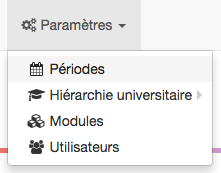
\includegraphics{menu_periode.png}}
\caption{Le menu permettant d'accéder à la gestion des périodes.}\end{figure}


\section{Définir les enseignements}
\label{admin:definir-les-enseignements}

\subsection{Créer les modules (unités d'enseignement)}
\label{admin:creer-les-modules-unites-d-enseignement}
Pour créer un module, depuis le tableau de bord, cliquer sur \textbf{voir les unités d'enseignement}, puis sur le bouton vert \textbf{+ nouveau module}, en haut, à droite de l'écran.

Il est également possible d'accéder aux modules depuis le menu \textbf{Paramètres} \textgreater{} \textbf{Modules}.
\begin{figure}[htbp]
\centering
\capstart

\scalebox{0.500000}{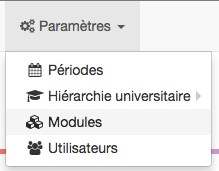
\includegraphics{menu_module.png}}
\caption{Le menu permettant d'accéder au paramétrage des modules.}\end{figure}

Les modules ou unités d'enseignement sont une simple coquille vide qui viendra contenir les groupes. Un module est simplement défini par un code module et un libellé.


\subsection{Associer des groupes aux modules}
\label{admin:associer-des-groupes-aux-modules}
Les modules sont composés de groupes. Les groupes peuvent-être associés à un ou plusieurs parcours et permettent de réserver un nombre de place (la capacité du groupe) pour l'ensemble des étudiant faisant partie des parcours.

Un groupe est associé à une période.

Depuis la liste des modules, il est possible de définir, pour chaque module, des groupes.
\begin{figure}[htbp]
\centering
\capstart

\scalebox{0.500000}{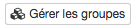
\includegraphics{gerer_groupe.png}}
\caption{Le bouton permettant d'accéder à la gestiond des groupes d'un module.}\end{figure}

Cliquez sur le bouton \textbf{Gérer les groupes} du module pour lequel vous souhaiter créer un/des groupes puis sur \textbf{+ Nouveau groupe}.

Vous pouvez créer autant de groupe que nécessaire par module.


\subsubsection{Notion de groupes obligatoires}
\label{admin:notion-de-groupes-obligatoires}
Si l'administrateur coche la case \textbf{Les étudiants associés aux parcours de ce groupe doivent-être obligatoirement présents}, il définit alors la présence des étudiants dans ce groupe comme \textbf{obligatoire}.

Lorsqu'un groupe est obligatoire, sa capacité n'est plus pertinente et — même si sa saisie reste obligatoire — elle ne sera pas prise en compte par l'application.

Un groupe \textbf{obligatoire} permet d'affecter de facto l'ensemble des étudiants enregistré dans les parcours associés au groupe obligatoire au groupe (et donc au module parent). De cette façon, l'application est capable de générer des feuilles d'émargement complètes pour les modules mixant présence optionnelle et présence obligatoire en fonction des parcours.


\section{Gérer les utilisateurs}
\label{admin:gerer-les-utilisateurs}
Vous pouvez accéder à la gestion des utilisateurs depuis le tableau de bord, en cliquant sur \textbf{voir les utilisateurs}.

Il est également possible d'accéder aux modules depuis le menu \textbf{Paramètres} \textgreater{} \textbf{Utilisateurs}.
\begin{figure}[htbp]
\centering
\capstart

\scalebox{0.500000}{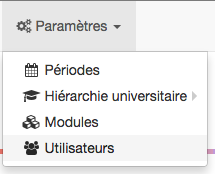
\includegraphics{menu_utilisateur.png}}
\caption{Le menu permettant d'accéder à la gestion des utilisateurs.}\end{figure}


\subsection{Filtres et tris}
\label{admin:filtres-et-tris}
L'application dispose de filtres sur tableaux qui vous permettent de filtrer rapidement et de rechercher des utilisateurs par saisie de leur prénom et/ou nom et par sélection du rôle, de la mention, de la spécialité ou du parcours.
\begin{figure}[htbp]
\centering
\capstart

\scalebox{0.800000}{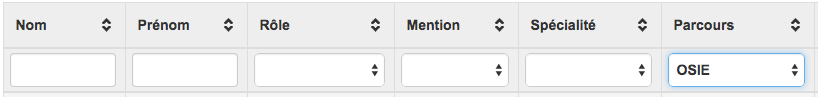
\includegraphics{filtres_tableaux.png}}
\caption{Le filtre sur tableau du module Utilisateurs.}\end{figure}

Vous pouvez également trier chaque colonne en faisant un simple clic pour un tri ascendant ou un double clic pour un tri descendant.


\subsection{Valider les utilisateurs}
\label{admin:valider-les-utilisateurs}
Lorsqu'un utilisateur s'inscrit, il est nécessaire de valider son compte afin que celui-ci puisse effectuer son choix d'options.

\begin{notice}{note}{Note:}
Tant que l'administrateur n'a pas validé les comptes des utilisateurs en attente de validation, ces derniers ne seront pas en mesure de se connecter à l'application et d'effectuer leur choix d'options.
\end{notice}

Si des utilisateurs sont en attente de validation, cela est signalé dans le tableau de bord par un encart rouge. Il suffit alors de cliquer sur \textbf{-\textgreater{} valider les utilisateurs en attente}.

Il est également possible d'accéder à l'écran de validation des utilisateurs par le menu \textbf{Paramètres} \textgreater{} \textbf{Utilisateurs} puis en cliquant sur le bouton vert, en haut, à droite ``Valider les utilisateurs''.

Pour valider les utilisateurs, sélectionnez les utilisateurs à valider en cochant les lignes souhaitées puis cliquez sur \textbf{Valider cocher}.

Si au contraire vous souhaiter supprimer les utilsiateurs cochés, cliquez sur \textbf{Supprimer cochés}.
\begin{figure}[htbp]
\centering
\capstart

\scalebox{0.800000}{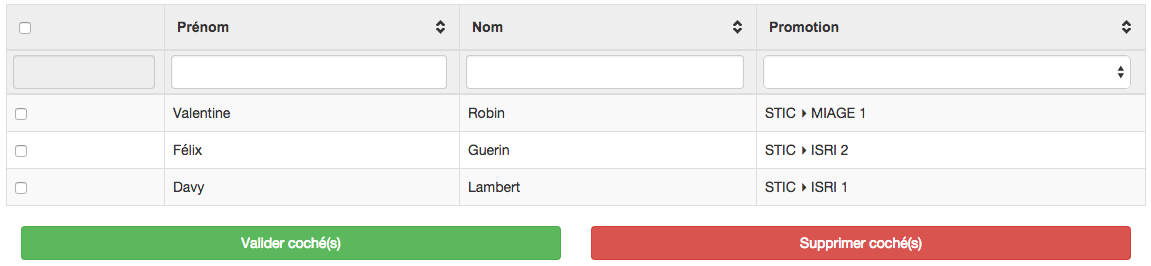
\includegraphics{validation_utilisateurs.png}}
\caption{Écran de validation ou suppression des comptes utilisateurs.}\end{figure}

Les filtres sur tableaux vous permettent de sélectionner facilement les utilsateurs que vous souhaitez valider ou supprimer.

Pour cocher l'ensemble des utilisateurs, cliquez sur la case à cocher dans l'en-tête sur tableau.

\begin{notice}{note}{Note:}
Si vous commencez par cocher l'ensemble des utilisateurs puis que vous appliquez un filtre, les utilisateurs ne répondant pas au critère de filtre seront automatiquement décochés de façon à ce que vous ne validier ou supprimiez pas de façon accidentelle des utilisateurs non souhaités.
\end{notice}


\subsection{Modifier le mot de passe d'un utilisateur}
\label{admin:modifier-le-mot-de-passe-d-un-utilisateur}
Pour modifier le mot de passe d'un utilisateur qui l'aurait oublié, commencez par afficher la liste des utilisateurs depuis le menu \textbf{Paramètres} \textgreater{} \textbf{Utilisateurs}.

Cherchez ensuite l'utilisateur par saisie de son nom à l'aide des filtres sur tableau puis cliquer sur le bouton \textbf{Voir}.

Cliquez sur \textbf{modifier mon profil} puis sur \textbf{modifier mot de passe}.

Saisir deux fois le nouveau mot de passe et valider.


\subsection{Consulter les choix d'un utilisateur}
\label{admin:consulter-les-choix-d-un-utilisateur}
Pour afficher les choix d'un utilisateur, commencez par afficher la liste des utilisateurs depuis le menu \textbf{Paramètres} \textgreater{} \textbf{Utilisateurs}.

Cherchez ensuite l'utilisateur par saisie de son nom à l'aide des filtres sur tableau puis cliquer sur le bouton \textbf{Voir}.

Les choix de l'utilisateur s'affichent dans la partie droite de l'écran.


\chapter{Documentation professeur/secrétariat}
\label{index:documentation-professeur-secretariat}
Les professeurs et/ou le secrétariat est amené à imprimer des feuilles d'émargement, à envoyer des emails aux utilisateurs et à consulter les choix d'optionnelles en vue de leur report dans le logiciel Apogée.


\section{Afficher la synthèse}
\label{prof:afficher-la-synthese}\label{prof::doc}
Pour accéder à la synthèse, cliquer sur le menu \textbf{Synthèse} dans la barre de menus.

Vous devez ensuite sélectionner le parcours à afficher. Les listes déroulantes sont dépendantes. Si vous modifiez la valeur d'une liste, la page se rechargera et vous pourrez sélectionner les informations liées à la liste précédente.

Quand vous avez sélectionné le parcours, indiquez si vous souhaitez une synthèse par groupe ou par étudiant.
\begin{figure}[htbp]
\centering
\capstart

\scalebox{0.800000}{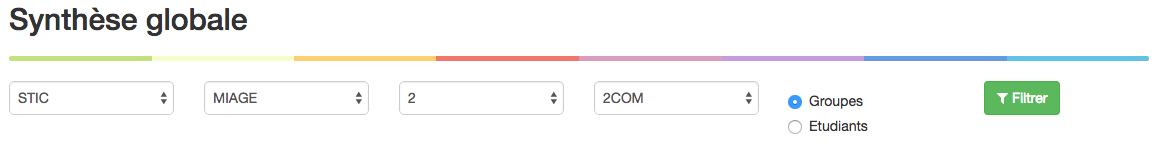
\includegraphics{synthese.png}}
\caption{Filtre permettant de sélectionner le parcours à afficher.}\end{figure}


\subsection{Synthèse par groupe}
\label{prof:synthese-par-groupe}
La vue groupe de la synthèse permet d'afficher l'ensembles des modules associés au parcours sélectionné.

Un clic sur le titre de chaque module permet d'afficher la liste des utilisateurs du parcours inscrits dans ce module.

Le badge présent à droite affiche le proportion que représente l'ensemble des étudiants du parcours sélectionné par rapport au nombre de places totales du groupe associé.
\begin{figure}[htbp]
\centering
\capstart

\scalebox{0.800000}{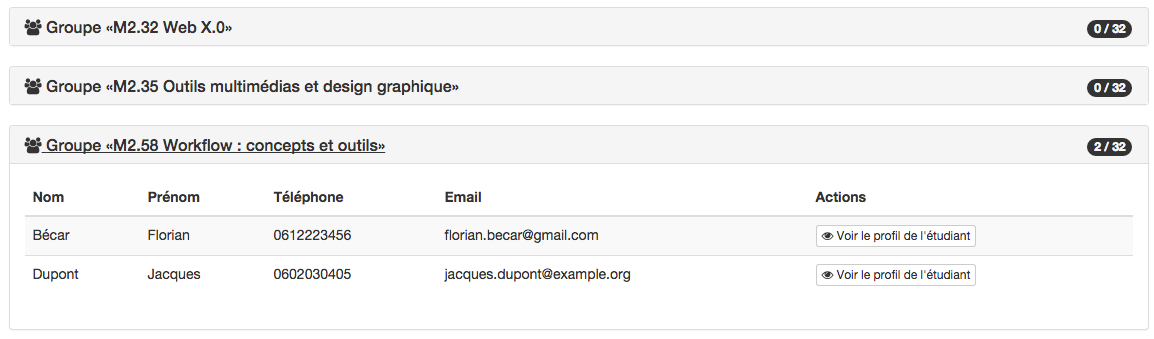
\includegraphics{synthese_groupe.png}}
\caption{Vue ``groupe'' de la synthèse.}\end{figure}


\subsection{Synthèse par utilisateur}
\label{prof:synthese-par-utilisateur}
La vue étudiant permet d'afficher l'ensemble des étudiants du parcours sélectionné, triés par ordre alphabétique
sur le nom.

Pour chaque étudiant, ses choix sont affichés.

Les modules obligatoires pour le parcours en cours sont rappelés dans la partie droite de l'écran.
\begin{figure}[htbp]
\centering
\capstart

\scalebox{0.800000}{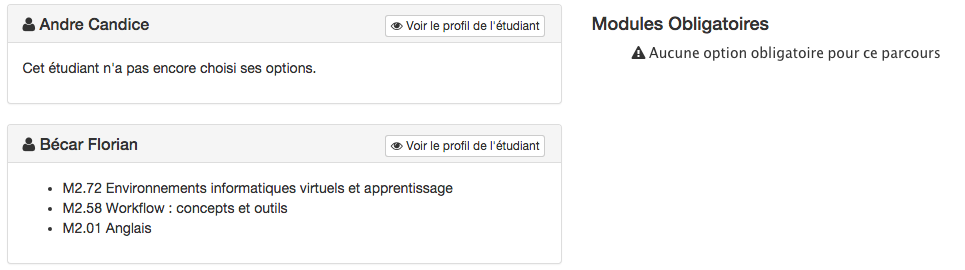
\includegraphics{synthese_etudiant.png}}
\caption{Vue ``étudiant'' de la synthèse.}\end{figure}


\section{Télécharger une feuille d'émargement}
\label{prof:telecharger-une-feuille-d-emargement}
Les feuilles d'émargement sont bien pratiques pour justifier de la présence des étudiants aux cours.

GICO est capable de générer des feuilles d'émargement qui combinent des étudiants de différents parcours et d'options obligatoire ou non. La solution est donc très flexible.

Depuis le tableau de bord, cliquer sur le pavé violet \textbf{accéder à la rubrique ``Au quotidien''}. Il est également possible de cliquer sur le menu \textbf{Au quotidien} dans la barre de menu de l'application.


\subsection{Par parcours}
\label{prof:par-parcours}
Pratique pour faire signer un groupe entier pour les enseignements ``classe complète'' de type ``Séminaires marchés professionels'', ``Amphithéâtres'', etc.

Les feuilles d'émargement par parcours sont situées dans la partie gauche de l'écran.


\subsubsection{Classeur (une feuille par parcours)}
\label{prof:classeur-une-feuille-par-parcours}
Pour télécharger un classeur Microsoft Excel contenant une feuille d'émargement par parcours, cliquez sur le bouton ``\textbf{Télécharger l'ensemble des feuilles}'' dans la partie gauche (\textbf{Parcours}) de l'écran.
\begin{figure}[htbp]
\centering
\capstart

\scalebox{0.500000}{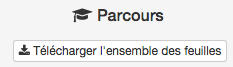
\includegraphics{emargement_parcours.png}}
\caption{Bouton permettant de télécharger les feuilles d'émargement de l'ensemble des parcours.}\end{figure}


\subsubsection{Feuille (un parcours)}
\label{prof:feuille-un-parcours}\begin{enumerate}
\item {} 
Dans la partie gauche de l'écran, cliquez sur le parcours dont vous souhaitez télécharger la feuille d'émargement pour faire apparaître les boutons d'options.

\item {} 
Cliquez ensuite sur \textbf{Télécharger la feuille d'émargement} pour télécharger la feuille d'émargement au format Microsoft Excel.

\end{enumerate}
\begin{figure}[htbp]
\centering
\capstart

\scalebox{0.500000}{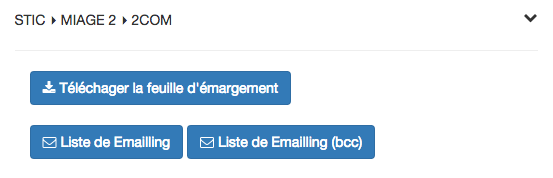
\includegraphics{un_parcours.png}}
\caption{Boutons d'actions permettant de télécharger la feuille d'émargement.}\end{figure}


\subsection{Par module}
\label{prof:par-module}
Pratique pour les cours mixant différents parcours et des types options/obligatoires selon le parcours.

Les feuilles d'émargement par modules sont situées dans la partie droite de l'écran.


\subsubsection{Classeur (tous les modules d'une promotion)}
\label{prof:classeur-tous-les-modules-d-une-promotion}\begin{enumerate}
\item {} 
Pour télécharger un classeur Microsoft Excel contenant une feuille d'émargement par module, pour une promotion donnée, commencez par sélectionner la promotion dans la liste déroulante, à droite de l'écran.

\item {} 
Cliquez sur le bouton ``\textbf{Télécharger l'ensemble des feuilles}'' dans la partie droite (\textbf{Modules}) de l'écran.

\end{enumerate}
\begin{figure}[htbp]
\centering
\capstart

\scalebox{0.500000}{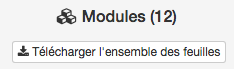
\includegraphics{emargement_modules.png}}
\caption{Bouton permettant de télécharger les feuilles d'émargement de l'ensemble des modules d'une promotion.}\end{figure}


\subsubsection{Feuille (un module)}
\label{prof:feuille-un-module}\begin{enumerate}
\item {} 
Dans la partie droite de l'écran, commencez par sélectionner la promotion dans laquelle se trouve le module dont vous souhaitez télécharger la feuille d'émargement.

\item {} 
Cliquez ensuite sur le titre du module dont vous souhaitez télécharger la feuille d'émargement pour faire apparaître les boutons d'options.

\item {} 
Enfin, cliquez sur \textbf{Télécharger la feuille d'émargement} pour télécharger la feuille d'émargement au format Microsoft Excel.

\end{enumerate}
\begin{figure}[htbp]
\centering
\capstart

\scalebox{0.500000}{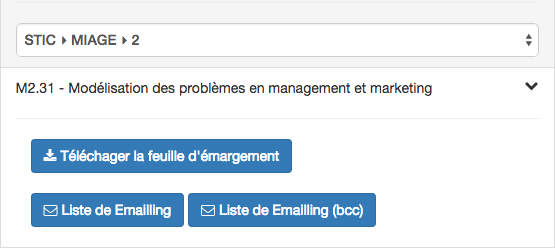
\includegraphics{un_module.png}}
\caption{Boutons d'actions permettant de télécharger la feuille d'émargement.}\end{figure}


\section{Envoyer un email groupé}
\label{prof:envoyer-un-email-groupe}
Les listes de Emailing permettent de récupérer simplement l'ensemble des mails des étudiants correspondant à un parcours ou un module.

Ainsi, plus la peine de submerger l'ensemble des étudiants de messages qui ne les concernent pas car ils n'ont pas choisi l'option associée.

Depuis le tableau de bord, cliquer sur le pavé violet \textbf{accéder à la rubrique ``Au quotidien''}. Il est également possible de cliquer sur le menu \textbf{Au quotidien} dans la barre de menu de l'application.


\subsection{Pour les étudiants d'un parcours}
\label{prof:pour-les-etudiants-d-un-parcours}\begin{enumerate}
\item {} 
Dans la partie gauche de l'écran, cliquez sur le parcours pour lequel vous souhaitez envoyer un email aux étudiants.

\item {} 
Cliquez ensuite sur \textbf{Liste de Emailing} pour envoyer un email à l'ensemble des étudiants du parcours correspondant (les différents emails des étudiants restent visibles — copie carbone) ou cliquez sur \textbf{Liste de Emailing (bcc)} pour envoyer l'email en copie carbone invisible (et ne pas divulguer les emails des étudiants).

\end{enumerate}
\begin{figure}[htbp]
\centering
\capstart

\scalebox{0.500000}{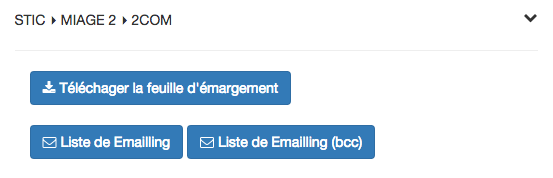
\includegraphics{un_parcours.png}}
\caption{Boutons d'actions permettant d'envoyer des emails.}\end{figure}


\subsection{Pour les étudiants d'un module}
\label{prof:pour-les-etudiants-d-un-module}\begin{enumerate}
\item {} 
Dans la partie droite de l'écran, commencez par sélectionner la promotion dans laquelle se trouve le module pour lequel vous souhaitez envoyer un email aux étudiants.

\item {} 
Cliquez ensuite sur \textbf{Liste de Emailing} pour envoyer un email à l'ensemble des étudiants du parcours correspondant (les différents emails des étudiants restent visibles — copie carbone) ou cliquez sur \textbf{Liste de Emailing (bcc)} pour envoyer l'email en copie carbone invisible (et ne pas divulguer les emails des étudiants).

\end{enumerate}
\begin{figure}[htbp]
\centering
\capstart

\scalebox{0.500000}{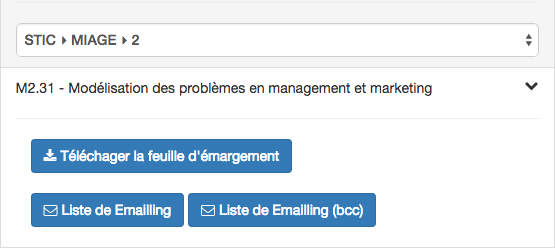
\includegraphics{un_module.png}}
\caption{Boutons d'actions permettant d'envoyer des emails.}\end{figure}


\chapter{Documentation utilisateur}
\label{index:documentation-utilisateur}
Il s'agit de l'étudiant qui effectue ses choix d'options.


\section{S'inscrire}
\label{etudiant:s-inscrire}\label{etudiant::doc}
La première étape pour pouvoir utiliser GICO est de s'inscrire en remplissant le formulaire d'inscription.

Dans la barre de menus, cliquer en haut, à droite sur \textbf{Inscription}.
\begin{figure}[htbp]
\centering
\capstart

\scalebox{0.500000}{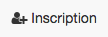
\includegraphics{inscription.png}}
\caption{Bouton permettant de s'inscrire.}\end{figure}

Remplir l'ensemble des champs, sélectionner le parcours et cliquer sur \textbf{Inscription}.

Attention à renseigner correctement l'email et le téléphone, ces informations étant utilisées par la scolarité.
\begin{figure}[htbp]
\centering
\capstart

\scalebox{0.500000}{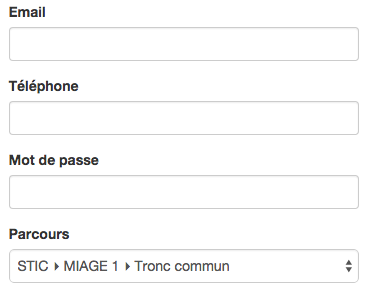
\includegraphics{champs_importants.png}}
\caption{Formulaire d'inscription.}\end{figure}

\begin{notice}{note}{Note:}
Attention, l'email et l'identifiant renseignés ne doivent pas déjà exister.
Si des erreurs sont rencontrés, elles vous seront signalées en rouge.
\end{notice}

Attendre l'activation de votre compte par l'administrateur.

Les comptes sont validés manuellement et l'activation peut donc prendre un certain temps.


\section{Se connecter}
\label{etudiant:se-connecter}
Une fois que l’administrateur aura validé votre compte, un mail vous sera envoyé pour vous le signaler et vous pourrez alors vous connecter pour procéder à la sélection de vos choix ou encore à la vérification ou à la modification de vos informations personnelles.

\begin{notice}{note}{Note:}
Gardez bien à l’esprit que ces informations que vous saisirez dans l’application seront un moyen pour l’administration de vous contacter. Il vaudrait donc mieux que ces dernières soient correctes.
\end{notice}

Pour vous connecter, il vous suffit de vous rendre sur le site de l’application, de cliquer sur le bouton ‘Connexion’ et d’entrer votre identifiant et votre mot de passe. Puis validez et vous serez enfin connecté.

\begin{notice}{note}{Note:}
Si vous tentez de vous connecter avec vos informations de connexion avant d’avoir reçu un mail signalant l’activation de votre compte alors votre tentative de connexion sera vaine. Nul besoin de s’inscrire de nouveau, attendez simplement le mail de confirmation d’activation de votre compte pour vous connecter.
\end{notice}


\section{Faire ses choix}
\label{etudiant:faire-ses-choix}
Pendant les date définies dans la période, vous pourrez vous inscrire à un nombre fini de modules optionnels. Attention , les places peuvent être limitées! Pour être sur de pouvoir vous inscrire aux cours que vous désirez, connectez vous le plus rapidement possible pendant la période de choix des options.

\begin{notice}{note}{Note:}
Pour chaque module, pous pouvez voir le nombre de places restantes dans le groupe signalées à droite du libellé du module.
\end{notice}

Cochez les cours qui vous intéressent puis validez.
\begin{figure}[htbp]
\centering
\capstart

\scalebox{0.700000}{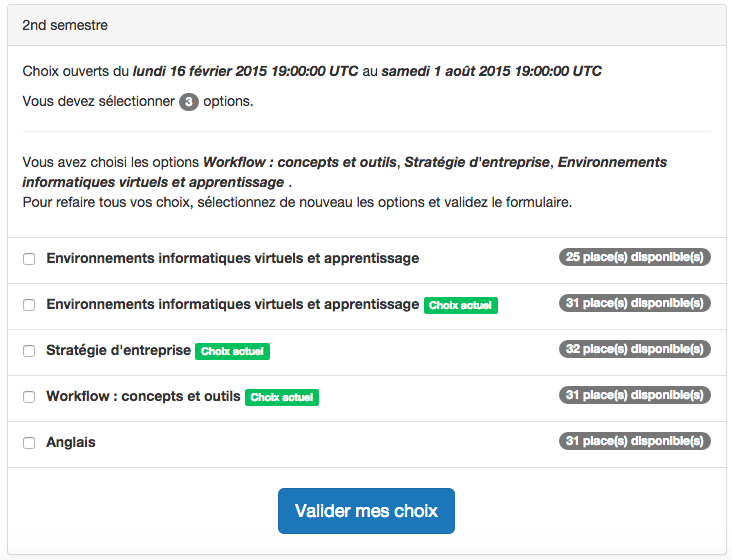
\includegraphics{faire_choix.png}}
\caption{Interface de saisie du choix.}\end{figure}

Voila, vous êtes désormais inscrit aux cours que vous avez choisi.

\begin{notice}{note}{Note:}
Vos choix actuels sont rappelés par une étiquette verte \textbf{Choix actuel} en regard des modules que vous avez choisi et les modules choisis sont rappelés en en-tête.
\end{notice}

Libre à vous de changer vos choix d’options durant la période de choix si vous le désirez en reselectionnant les options que vous souhaitez suivre.



\renewcommand{\indexname}{Index}
\printindex
\end{document}
